% Options for packages loaded elsewhere
\PassOptionsToPackage{unicode}{hyperref}
\PassOptionsToPackage{hyphens}{url}
\documentclass[
]{article}
\usepackage{xcolor}
\usepackage[margin=24mm]{geometry}
\usepackage{amsmath,amssymb}
\setcounter{secnumdepth}{-\maxdimen} % remove section numbering
\usepackage{iftex}
\ifPDFTeX
  \usepackage[T1]{fontenc}
  \usepackage[utf8]{inputenc}
  \usepackage{textcomp} % provide euro and other symbols
\else % if luatex or xetex
  \usepackage{unicode-math} % this also loads fontspec
  \defaultfontfeatures{Scale=MatchLowercase}
  \defaultfontfeatures[\rmfamily]{Ligatures=TeX,Scale=1}
\fi
\usepackage{lmodern}
\ifPDFTeX\else
  % xetex/luatex font selection
\fi
% Use upquote if available, for straight quotes in verbatim environments
\IfFileExists{upquote.sty}{\usepackage{upquote}}{}
\IfFileExists{microtype.sty}{% use microtype if available
  \usepackage[]{microtype}
  \UseMicrotypeSet[protrusion]{basicmath} % disable protrusion for tt fonts
}{}
\makeatletter
\@ifundefined{KOMAClassName}{% if non-KOMA class
  \IfFileExists{parskip.sty}{%
    \usepackage{parskip}
  }{% else
    \setlength{\parindent}{0pt}
    \setlength{\parskip}{6pt plus 2pt minus 1pt}}
}{% if KOMA class
  \KOMAoptions{parskip=half}}
\makeatother
\usepackage{color}
\usepackage{fancyvrb}
\newcommand{\VerbBar}{|}
\newcommand{\VERB}{\Verb[commandchars=\\\{\}]}
\DefineVerbatimEnvironment{Highlighting}{Verbatim}{commandchars=\\\{\}}
% Add ',fontsize=\small' for more characters per line
\newenvironment{Shaded}{}{}
\newcommand{\AlertTok}[1]{\textcolor[rgb]{1.00,0.00,0.00}{\textbf{#1}}}
\newcommand{\AnnotationTok}[1]{\textcolor[rgb]{0.38,0.63,0.69}{\textbf{\textit{#1}}}}
\newcommand{\AttributeTok}[1]{\textcolor[rgb]{0.49,0.56,0.16}{#1}}
\newcommand{\BaseNTok}[1]{\textcolor[rgb]{0.25,0.63,0.44}{#1}}
\newcommand{\BuiltInTok}[1]{\textcolor[rgb]{0.00,0.50,0.00}{#1}}
\newcommand{\CharTok}[1]{\textcolor[rgb]{0.25,0.44,0.63}{#1}}
\newcommand{\CommentTok}[1]{\textcolor[rgb]{0.38,0.63,0.69}{\textit{#1}}}
\newcommand{\CommentVarTok}[1]{\textcolor[rgb]{0.38,0.63,0.69}{\textbf{\textit{#1}}}}
\newcommand{\ConstantTok}[1]{\textcolor[rgb]{0.53,0.00,0.00}{#1}}
\newcommand{\ControlFlowTok}[1]{\textcolor[rgb]{0.00,0.44,0.13}{\textbf{#1}}}
\newcommand{\DataTypeTok}[1]{\textcolor[rgb]{0.56,0.13,0.00}{#1}}
\newcommand{\DecValTok}[1]{\textcolor[rgb]{0.25,0.63,0.44}{#1}}
\newcommand{\DocumentationTok}[1]{\textcolor[rgb]{0.73,0.13,0.13}{\textit{#1}}}
\newcommand{\ErrorTok}[1]{\textcolor[rgb]{1.00,0.00,0.00}{\textbf{#1}}}
\newcommand{\ExtensionTok}[1]{#1}
\newcommand{\FloatTok}[1]{\textcolor[rgb]{0.25,0.63,0.44}{#1}}
\newcommand{\FunctionTok}[1]{\textcolor[rgb]{0.02,0.16,0.49}{#1}}
\newcommand{\ImportTok}[1]{\textcolor[rgb]{0.00,0.50,0.00}{\textbf{#1}}}
\newcommand{\InformationTok}[1]{\textcolor[rgb]{0.38,0.63,0.69}{\textbf{\textit{#1}}}}
\newcommand{\KeywordTok}[1]{\textcolor[rgb]{0.00,0.44,0.13}{\textbf{#1}}}
\newcommand{\NormalTok}[1]{#1}
\newcommand{\OperatorTok}[1]{\textcolor[rgb]{0.40,0.40,0.40}{#1}}
\newcommand{\OtherTok}[1]{\textcolor[rgb]{0.00,0.44,0.13}{#1}}
\newcommand{\PreprocessorTok}[1]{\textcolor[rgb]{0.74,0.48,0.00}{#1}}
\newcommand{\RegionMarkerTok}[1]{#1}
\newcommand{\SpecialCharTok}[1]{\textcolor[rgb]{0.25,0.44,0.63}{#1}}
\newcommand{\SpecialStringTok}[1]{\textcolor[rgb]{0.73,0.40,0.53}{#1}}
\newcommand{\StringTok}[1]{\textcolor[rgb]{0.25,0.44,0.63}{#1}}
\newcommand{\VariableTok}[1]{\textcolor[rgb]{0.10,0.09,0.49}{#1}}
\newcommand{\VerbatimStringTok}[1]{\textcolor[rgb]{0.25,0.44,0.63}{#1}}
\newcommand{\WarningTok}[1]{\textcolor[rgb]{0.38,0.63,0.69}{\textbf{\textit{#1}}}}
\usepackage{longtable,booktabs,array}
\newcounter{none} % for unnumbered tables
\usepackage{calc} % for calculating minipage widths
% Correct order of tables after \paragraph or \subparagraph
\usepackage{etoolbox}
\makeatletter
\patchcmd\longtable{\par}{\if@noskipsec\mbox{}\fi\par}{}{}
\makeatother
% Allow footnotes in longtable head/foot
\IfFileExists{footnotehyper.sty}{\usepackage{footnotehyper}}{\usepackage{footnote}}
\makesavenoteenv{longtable}
\usepackage{graphicx}
\makeatletter
\newsavebox\pandoc@box
\newcommand*\pandocbounded[1]{% scales image to fit in text height/width
  \sbox\pandoc@box{#1}%
  \Gscale@div\@tempa{\textheight}{\dimexpr\ht\pandoc@box+\dp\pandoc@box\relax}%
  \Gscale@div\@tempb{\linewidth}{\wd\pandoc@box}%
  \ifdim\@tempb\p@<\@tempa\p@\let\@tempa\@tempb\fi% select the smaller of both
  \ifdim\@tempa\p@<\p@\scalebox{\@tempa}{\usebox\pandoc@box}%
  \else\usebox{\pandoc@box}%
  \fi%
}
% Set default figure placement to htbp
\def\fps@figure{htbp}
\makeatother
\setlength{\emergencystretch}{3em} % prevent overfull lines
\providecommand{\tightlist}{%
  \setlength{\itemsep}{0pt}\setlength{\parskip}{0pt}}
\usepackage{bookmark}
\IfFileExists{xurl.sty}{\usepackage{xurl}}{} % add URL line breaks if available
\urlstyle{same}
\hypersetup{
  hidelinks,
  pdfcreator={LaTeX via pandoc}}

\author{}
\date{}

\begin{document}

\section{Preliminary Summary of Distance-Exponent Readout by Independent
Metric C and Relational Compensation Decomposition in an ABC Closed
Phase
System}\label{preliminary-summary-of-distance-exponent-readout-by-independent-metric-c-and-relational-compensation-decomposition-in-an-abc-closed-phase-system}

\textbf{Date:} 2026-07-12\\
\textbf{Author:} Noriaki Kihara\\
\textbf{Position:} Summary of the ABC distance-exponent preliminary
experiment group in the Wave Information Readout series\\
\textbf{Version DOI:} 10.5281/zenodo.21318701\\
\textbf{Concept DOI:} 10.5281/zenodo.21318700

\begin{center}\rule{0.5\linewidth}{0.5pt}\end{center}

\subsection{Abstract}\label{abstract}

This summary consolidates a group of preliminary ABC closed phase system
experiments introduced after the AB two-body system failed to determine
the distance exponent independently.

The target experiments are:

\begin{enumerate}
\def\labelenumi{\arabic{enumi}.}
\tightlist
\item
  distance-exponent readout of AB relational compensation using an
  independent metric C,
\item
  C-position control for distance-exponent readout, and
\item
  relational compensation decomposition.
\end{enumerate}

The conclusion is:

\begin{Shaded}
\begin{Highlighting}[]
\NormalTok{To address the distance{-}exponent question left open by the AB two{-}body problem,}
\NormalTok{the measuring wave C was placed inside the same closed phase system.}

\NormalTok{Even in this ABC three{-}body system, the acceleration{-}like AB relational compensation can be read.}

\NormalTok{However, no inverse{-}law or inverse{-}square{-}law dependence on position phase difference was observed.}
\end{Highlighting}
\end{Shaded}

In valid gauge cases, the recovered exponent was mainly

\begin{Shaded}
\begin{Highlighting}[]
\NormalTok{alpha ≈ {-}1.}
\end{Highlighting}
\end{Shaded}

Since the experiments classify the readout as

\begin{Shaded}
\begin{Highlighting}[]
\NormalTok{I\_AB(L) proportional to L\^{}\{{-}alpha\},}
\end{Highlighting}
\end{Shaded}

\texttt{alpha≈-1} means

\begin{Shaded}
\begin{Highlighting}[]
\NormalTok{I\_AB(L) proportional to L.}
\end{Highlighting}
\end{Shaded}

That is, the result is proportional-type.

This is interpreted as a consequence of the fact that the present
experiment is essentially a one-dimensional harmonic-oscillation model
made of two localized waves imitating localized particles.

Within this model, effects of relative distance are not received, or
even if they are received, they cannot be observed.

In particular, although C was introduced as an independent metric gauge,
C is itself part of the closed phase system and therefore cannot be an
absolute external gauge.

Thus, even after adding C, the proportional type remained within the
current model.

This does not generally deny inverse-square behavior.

The narrower claim that was not supported is:

\begin{Shaded}
\begin{Highlighting}[]
\NormalTok{An inverse{-}law or inverse{-}square{-}law relation appears natively}
\NormalTok{from the present one{-}dimensional AB harmonic model plus the C metric gauge.}
\end{Highlighting}
\end{Shaded}

The possibility of extending the position phase degrees of freedom to
three or four dimensions was considered. However, as long as the same
localized two-wave harmonic model is used, any higher-dimensional
configuration returns to the same structure when projected onto a
geodesic or two-dimensional section. Therefore, this experiment group
did not proceed to three- or four-dimensional extensions at this stage.

\textbf{Keywords:} ABC closed phase system, independent metric C,
distance exponent, relational compensation decomposition,
\texttt{f\_AB}, \texttt{f\_AC}, \texttt{f\_BC}, \texttt{f\_ABC},
harmonic readout, inverse-square non-detection

\begin{center}\rule{0.5\linewidth}{0.5pt}\end{center}

\subsection{1. Experiment List}\label{experiment-list}

{\def\LTcaptype{none} % do not increment counter
\begin{longtable}[]{@{}
  >{\raggedleft\arraybackslash}p{(\linewidth - 6\tabcolsep) * \real{0.3077}}
  >{\raggedright\arraybackslash}p{(\linewidth - 6\tabcolsep) * \real{0.2308}}
  >{\raggedright\arraybackslash}p{(\linewidth - 6\tabcolsep) * \real{0.2308}}
  >{\raggedright\arraybackslash}p{(\linewidth - 6\tabcolsep) * \real{0.2308}}@{}}
\toprule\noalign{}
\begin{minipage}[b]{\linewidth}\raggedleft
No.
\end{minipage} & \begin{minipage}[b]{\linewidth}\raggedright
Experiment
\end{minipage} & \begin{minipage}[b]{\linewidth}\raggedright
Purpose
\end{minipage} & \begin{minipage}[b]{\linewidth}\raggedright
Main result
\end{minipage} \\
\midrule\noalign{}
\endhead
\bottomrule\noalign{}
\endlastfoot
1 & C-gauge valid-window test & Test whether \texttt{C} can serve as an
independent metric for AB distance exponent & Valid window exists \\
2 & C-position control & Test whether
symmetric/asymmetric/phase-inverted C changes the exponent &
Proportional type remained \\
3 & Relational compensation decomposition & Separate \texttt{f\_AB},
\texttt{f\_AC}, \texttt{f\_BC}, and \texttt{f\_ABC} & Separation rule
supported \\
\end{longtable}
}

\begin{center}\rule{0.5\linewidth}{0.5pt}\end{center}

\subsection{2. Distance-Exponent Readout Using Independent Metric
C}\label{distance-exponent-readout-using-independent-metric-c}

\subsubsection{2.1 Meaning of the
Experiment}\label{meaning-of-the-experiment}

In the AB two-body system alone, it was possible to read that

\begin{Shaded}
\begin{Highlighting}[]
\NormalTok{relative distance changed.}
\end{Highlighting}
\end{Shaded}

However, there was no independent gauge for deciding whether the change
should be measured as proportional, inverse proportional, or
inverse-square.

Therefore, a third wave \texttt{C} was placed and tested as a metric
gauge for reading the position-change and temporal-phase-change
quantities of AB.

The following were not implemented:

\begin{Shaded}
\begin{Highlighting}[]
\NormalTok{1/L\_AB}
\NormalTok{1/L\_AB\^{}2}
\NormalTok{1/A\_chi\_tau}
\NormalTok{F = G m\_A m\_B / L\_AB\^{}2}
\end{Highlighting}
\end{Shaded}

Thus, if an inverse-law or inverse-square-law form appears, it must be a
result of C-gauge readout rather than a constructed implementation.

\subsubsection{2.2 Main Result}\label{main-result}

{\def\LTcaptype{none} % do not increment counter
\begin{longtable}[]{@{}lr@{}}
\toprule\noalign{}
Quantity & Value \\
\midrule\noalign{}
\endhead
\bottomrule\noalign{}
\endlastfoot
\texttt{config\_count} & \texttt{160} \\
\texttt{gauge\_valid\_count} & \texttt{41} \\
\texttt{resolution\_valid\_count} & \texttt{60} \\
\texttt{clock\_valid\_count} & \texttt{100} \\
\texttt{disturbance\_valid\_count} & \texttt{101} \\
\texttt{inverse\_like\_alpha1\_count} & \texttt{0} \\
\texttt{inverse\_square\_like\_alpha2\_count} & \texttt{0} \\
\texttt{proportional\_like\_alpha\_minus1\_count} & \texttt{41} \\
\texttt{alpha\_min} & \texttt{-1.0000000000000002} \\
\texttt{alpha\_max} & \texttt{-0.9569628567496087} \\
\end{longtable}
}

The classification by relational time was:

{\def\LTcaptype{none} % do not increment counter
\begin{longtable}[]{@{}ll@{}}
\toprule\noalign{}
Time candidate & Classification \\
\midrule\noalign{}
\endhead
\bottomrule\noalign{}
\endlastfoot
\texttt{tau\_ABC} & \texttt{proportional\_like\_alpha\_minus1\ =\ 41} \\
\texttt{tau\_AB} & \texttt{other\ =\ 41} \\
\texttt{tau\_AC} & \texttt{proportional\_like\_alpha\_minus1\ =\ 41} \\
\texttt{tau\_BC} & \texttt{proportional\_like\_alpha\_minus1\ =\ 41} \\
\end{longtable}
}

\texttt{tau\_AB} deviated from \texttt{tau\_ABC} by up to about
\texttt{0.659}.

Therefore, reading the distance exponent requires explicitly specifying

\begin{Shaded}
\begin{Highlighting}[]
\NormalTok{what is read as time.}
\end{Highlighting}
\end{Shaded}

\subsubsection{2.3 C-Gauge Valid Window}\label{c-gauge-valid-window}

In this experiment, \texttt{R\_C} was also treated as the metric-cell
density of C.

That is,

\begin{Shaded}
\begin{Highlighting}[]
\NormalTok{small R\_C}
\NormalTok{= low frequency of C}
\NormalTok{= long wavelength of C}
\NormalTok{= wide cell interval of C.}
\end{Highlighting}
\end{Shaded}

If \texttt{R\_C} is too small, C cannot read the AB position-change
quantity across multiple cells.

If \texttt{R\_C} becomes large, resolution improves, but the C-derived
relations \texttt{f\_AC}, \texttt{f\_BC}, and \texttt{f\_ABC}
contaminate the main AB readout.

Therefore, C has a valid window:

\begin{Shaded}
\begin{Highlighting}[]
\NormalTok{not too coarse, not too strong.}
\end{Highlighting}
\end{Shaded}

\subsubsection{2.4 Figures}\label{figures}

{\def\LTcaptype{none} % do not increment counter
\begin{longtable}[]{@{}
  >{\raggedright\arraybackslash}p{(\linewidth - 2\tabcolsep) * \real{0.5000}}
  >{\raggedright\arraybackslash}p{(\linewidth - 2\tabcolsep) * \real{0.5000}}@{}}
\toprule\noalign{}
\begin{minipage}[b]{\linewidth}\raggedright
C-gauge eligibility
\end{minipage} & \begin{minipage}[b]{\linewidth}\raggedright
Alpha candidates
\end{minipage} \\
\midrule\noalign{}
\endhead
\bottomrule\noalign{}
\endlastfoot
\pandocbounded{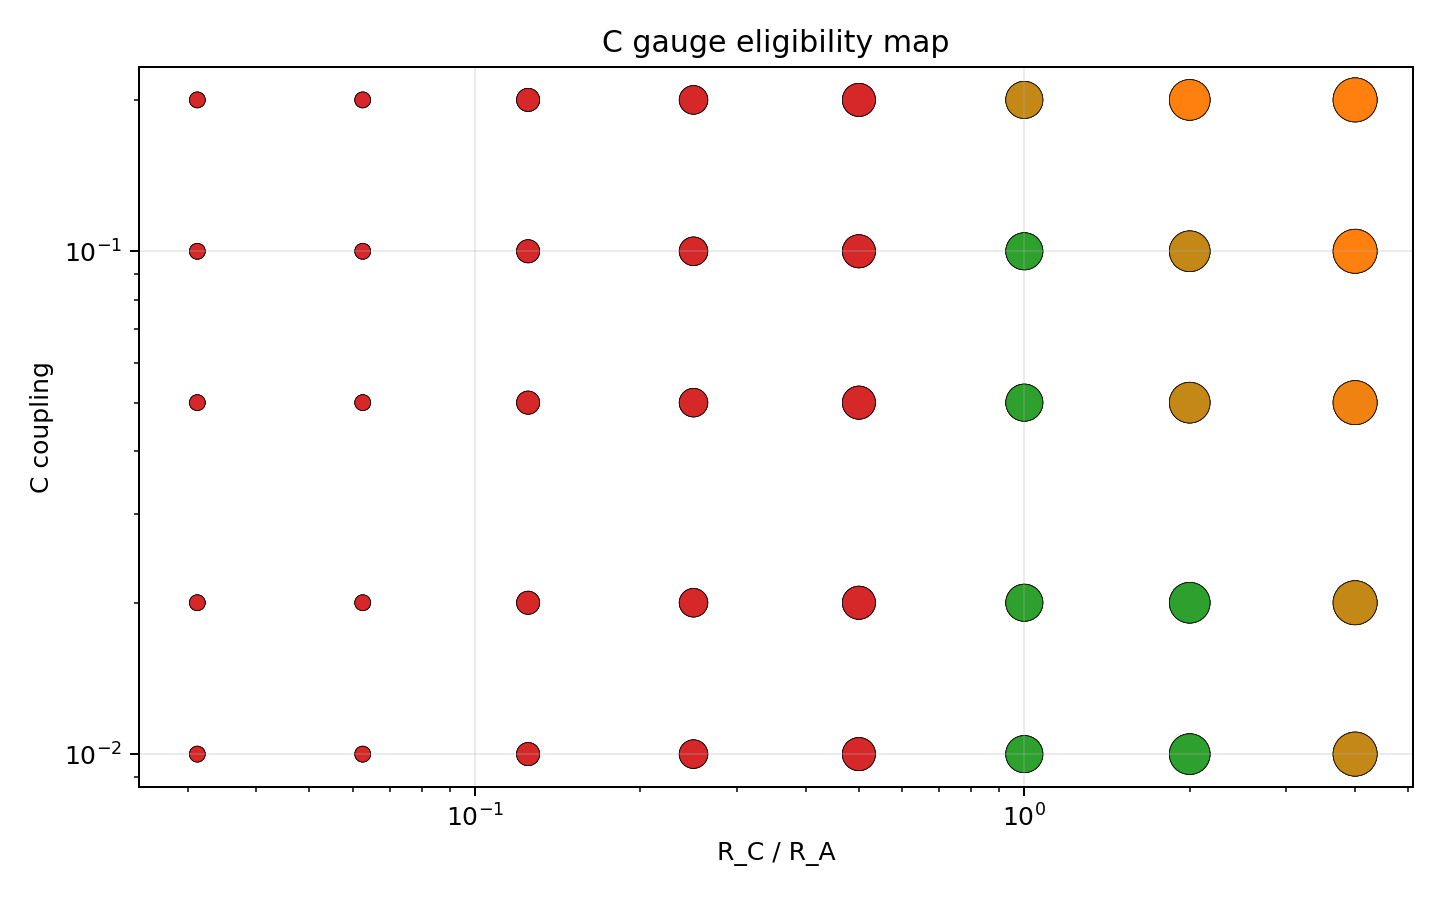
\includegraphics[keepaspectratio]{abc_c_gauge_ab_distance_exponent_preliminary_result_v1/abc_c_gauge_ab_distance_exponent_gauge_eligibility_map_v1.png}}
&
\pandocbounded{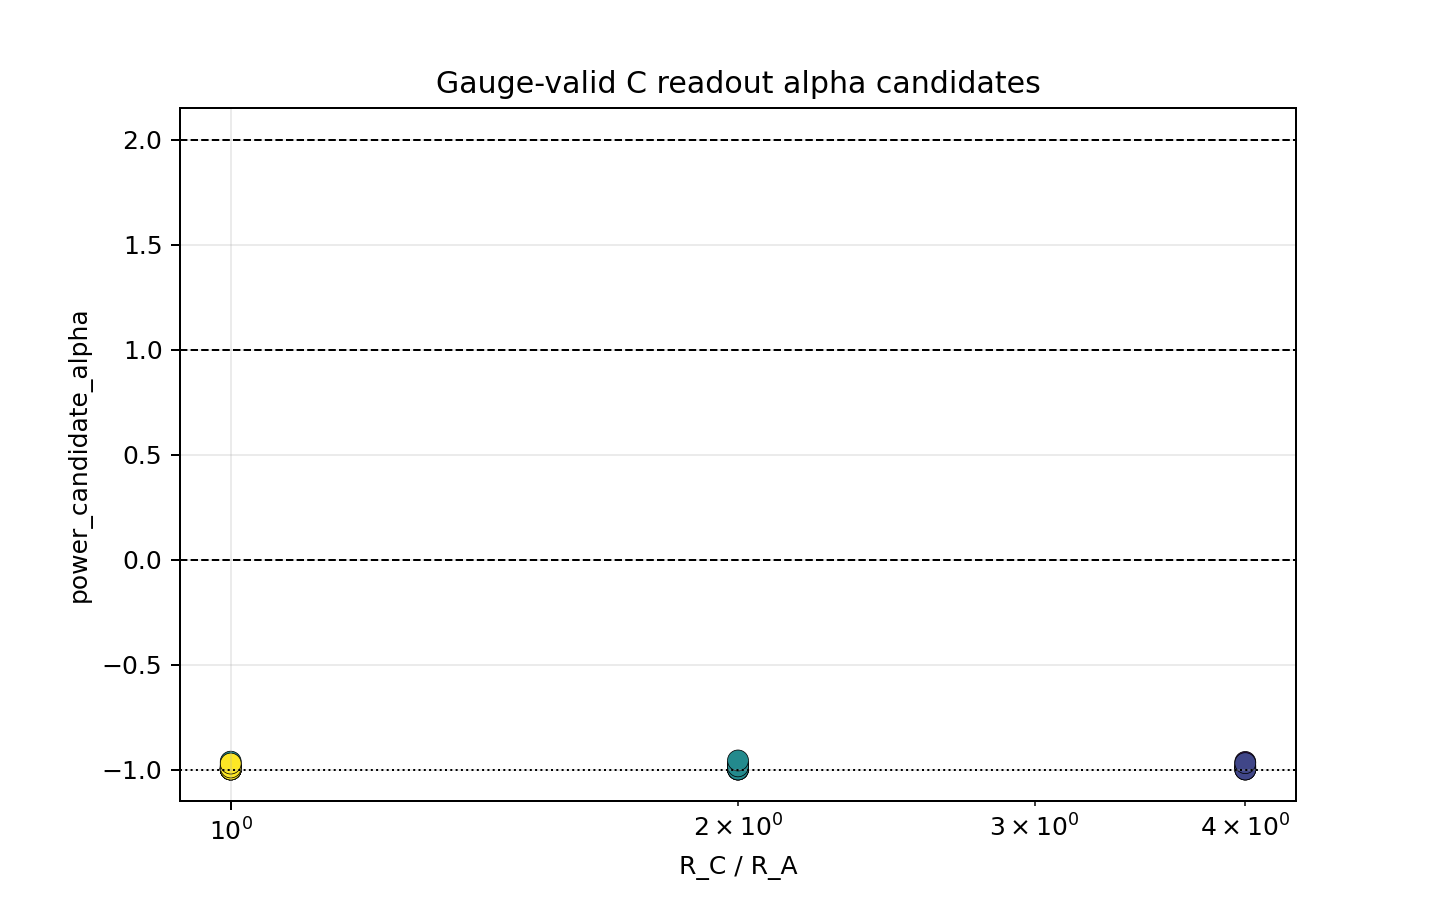
\includegraphics[keepaspectratio]{abc_c_gauge_ab_distance_exponent_preliminary_result_v1/abc_c_gauge_ab_distance_exponent_alpha_candidates_v1.png}} \\
\end{longtable}
}

{\def\LTcaptype{none} % do not increment counter
\begin{longtable}[]{@{}
  >{\raggedright\arraybackslash}p{(\linewidth - 2\tabcolsep) * \real{0.5000}}
  >{\raggedright\arraybackslash}p{(\linewidth - 2\tabcolsep) * \real{0.5000}}@{}}
\toprule\noalign{}
\begin{minipage}[b]{\linewidth}\raggedright
Reference curve
\end{minipage} & \begin{minipage}[b]{\linewidth}\raggedright
Filter diagnosis
\end{minipage} \\
\midrule\noalign{}
\endhead
\bottomrule\noalign{}
\endlastfoot
\pandocbounded{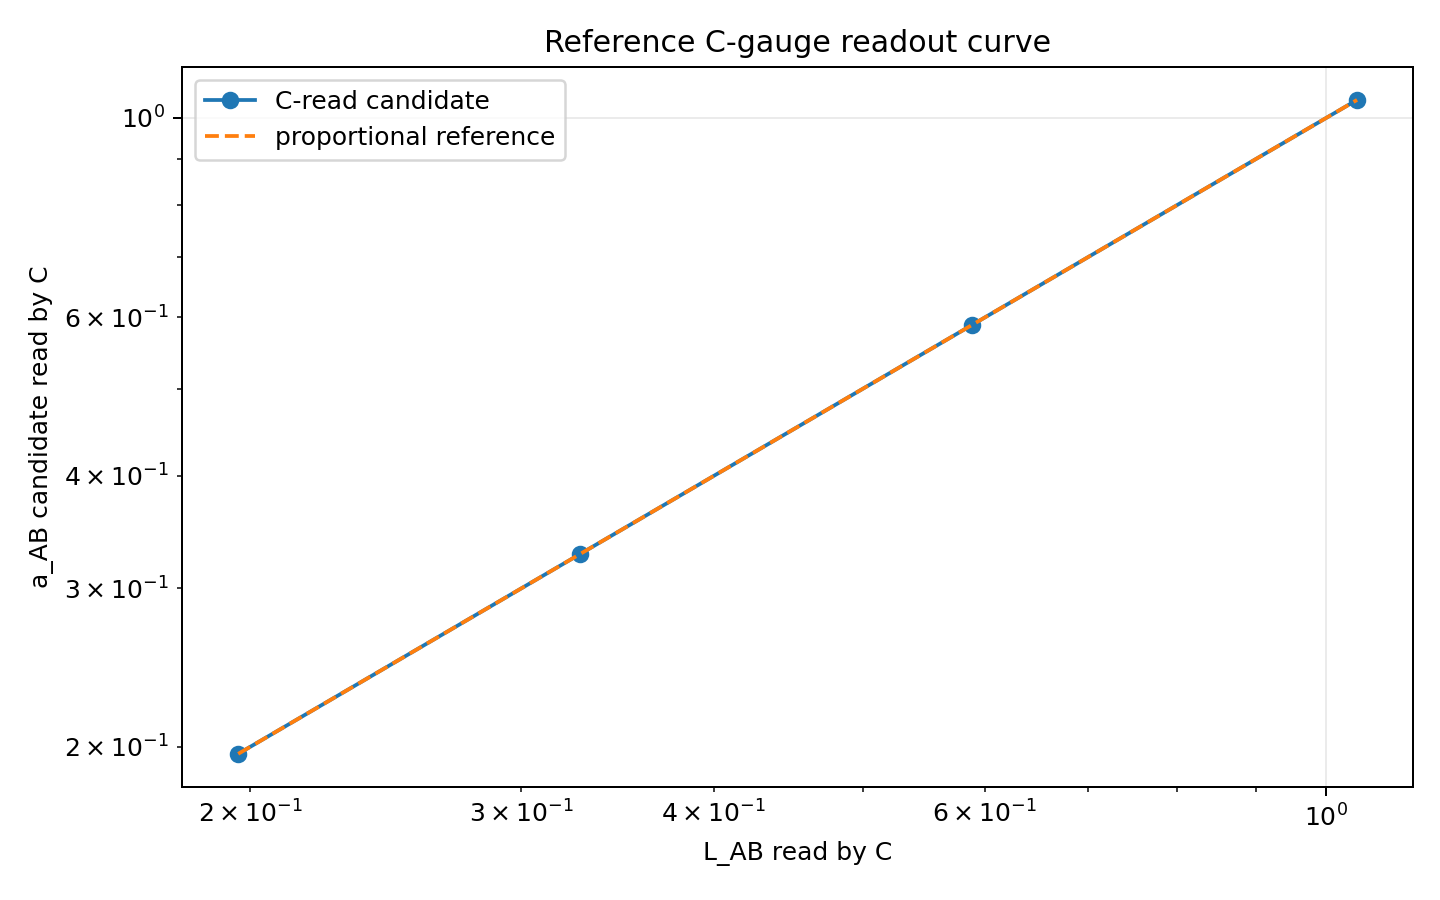
\includegraphics[keepaspectratio]{abc_c_gauge_ab_distance_exponent_preliminary_result_v1/abc_c_gauge_ab_distance_exponent_reference_curve_v1.png}}
&
\pandocbounded{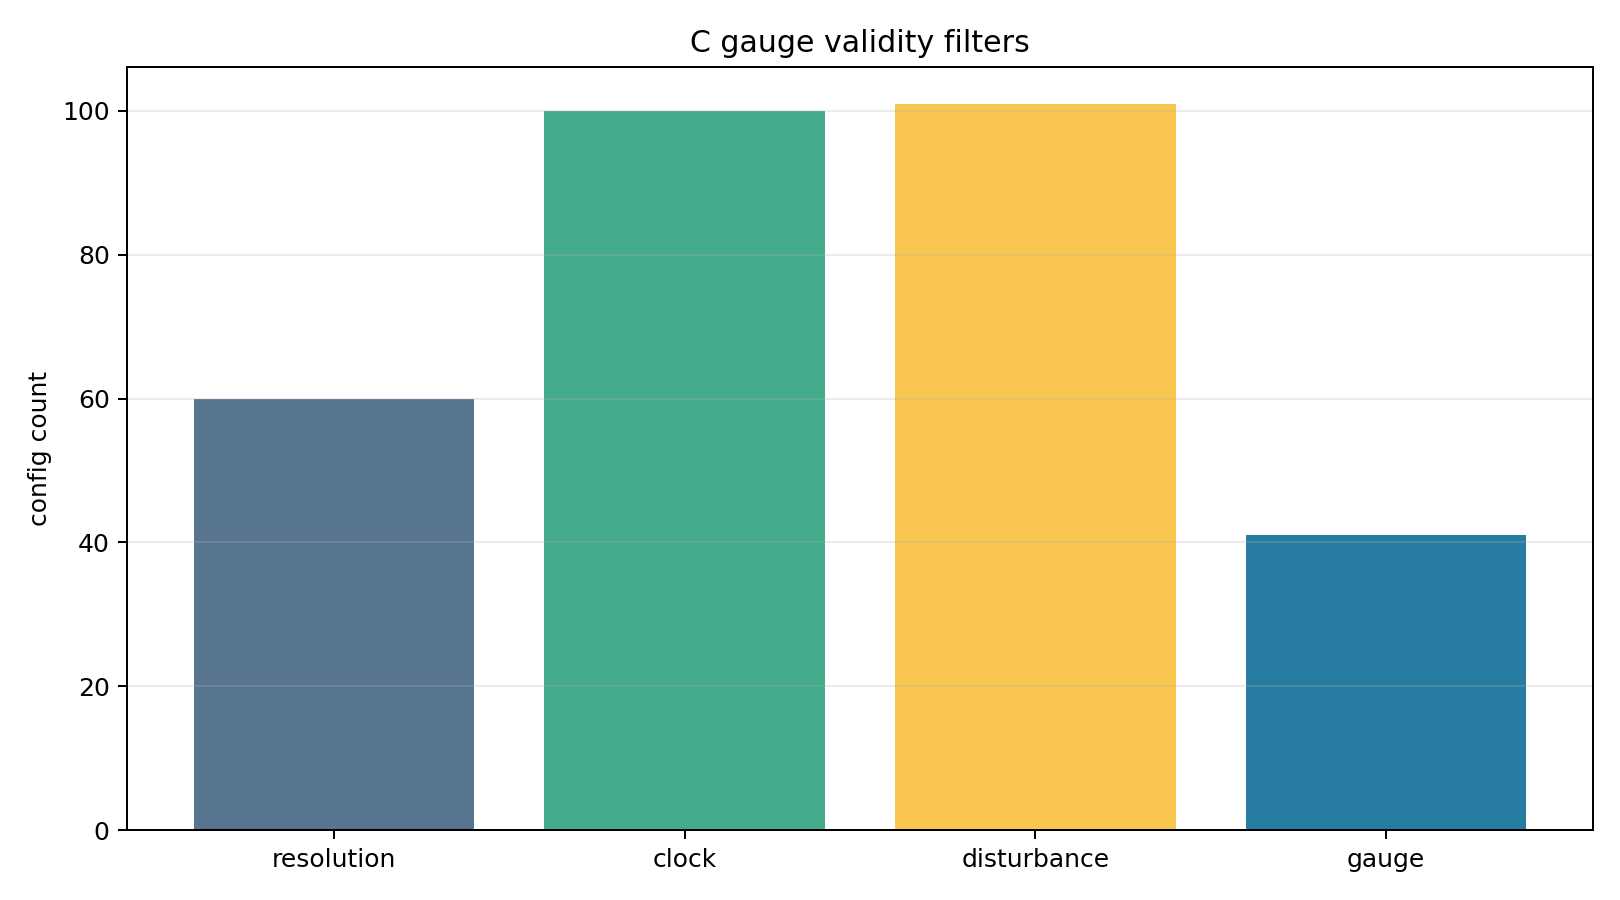
\includegraphics[keepaspectratio]{abc_c_gauge_ab_distance_exponent_preliminary_result_v1/abc_c_gauge_ab_distance_exponent_validity_filters_v1.png}} \\
\end{longtable}
}

\begin{center}\rule{0.5\linewidth}{0.5pt}\end{center}

\subsection{3. C-Position Control}\label{c-position-control}

\subsubsection{3.1 Meaning of the
Experiment}\label{meaning-of-the-experiment-1}

The third wave \texttt{C} is not an external observer. It is part of the
closed phase system.

Thus, placing C simultaneously generates

\begin{Shaded}
\begin{Highlighting}[]
\NormalTok{f\_AC}
\NormalTok{f\_BC}
\NormalTok{f\_ABC.}
\end{Highlighting}
\end{Shaded}

The experiment changed the position of C to test whether

\begin{Shaded}
\begin{Highlighting}[]
\NormalTok{the distance exponent changes,}
\NormalTok{or only the valid gauge window narrows due to contamination from C.}
\end{Highlighting}
\end{Shaded}

\subsubsection{3.2 C-Position Modes}\label{c-position-modes}

The compared positions were:

\begin{Shaded}
\begin{Highlighting}[]
\NormalTok{symmetric}
\NormalTok{symmetric\_pi\_flip}
\NormalTok{a\_side\_small}
\NormalTok{b\_side\_small}
\NormalTok{a\_side\_large}
\NormalTok{b\_side\_large}
\NormalTok{a\_side\_large\_pi\_flip}
\NormalTok{b\_side\_large\_pi\_flip}
\end{Highlighting}
\end{Shaded}

\subsubsection{3.3 Main Result}\label{main-result-1}

{\def\LTcaptype{none} % do not increment counter
\begin{longtable}[]{@{}
  >{\raggedright\arraybackslash}p{(\linewidth - 2\tabcolsep) * \real{0.4286}}
  >{\raggedleft\arraybackslash}p{(\linewidth - 2\tabcolsep) * \real{0.5714}}@{}}
\toprule\noalign{}
\begin{minipage}[b]{\linewidth}\raggedright
Quantity
\end{minipage} & \begin{minipage}[b]{\linewidth}\raggedleft
Value
\end{minipage} \\
\midrule\noalign{}
\endhead
\bottomrule\noalign{}
\endlastfoot
\texttt{config\_count} & \texttt{160} \\
\texttt{gauge\_valid\_count} & \texttt{70} \\
\texttt{gauge\_valid\_position\_pair\_count} & \texttt{23} \\
\texttt{max\_pair\_abs\_alpha\_difference} &
\texttt{0.11776992863447344} \\
Main classification under \texttt{tau\_ABC} &
\texttt{proportional\_like\_alpha\_minus1\ =\ 70} \\
\end{longtable}
}

The number of valid gauges by C-position mode was:

{\def\LTcaptype{none} % do not increment counter
\begin{longtable}[]{@{}lr@{}}
\toprule\noalign{}
C position & Valid count \\
\midrule\noalign{}
\endhead
\bottomrule\noalign{}
\endlastfoot
\texttt{symmetric} & \texttt{12} \\
\texttt{symmetric\_pi\_flip} & \texttt{12} \\
\texttt{a\_side\_small} & \texttt{11} \\
\texttt{b\_side\_small} & \texttt{11} \\
\texttt{a\_side\_large} & \texttt{6} \\
\texttt{b\_side\_large} & \texttt{6} \\
\texttt{a\_side\_large\_pi\_flip} & \texttt{6} \\
\texttt{b\_side\_large\_pi\_flip} & \texttt{6} \\
\end{longtable}
}

Large asymmetric C placement reduced the number of valid cases.

It is safer to read this not as the appearance of a new stable distance
exponent, but as:

\begin{Shaded}
\begin{Highlighting}[]
\NormalTok{bias in f\_AC and f\_BC narrowed the validity conditions of the C gauge.}
\end{Highlighting}
\end{Shaded}

\subsubsection{3.4 Figures}\label{figures-1}

{\def\LTcaptype{none} % do not increment counter
\begin{longtable}[]{@{}
  >{\raggedright\arraybackslash}p{(\linewidth - 2\tabcolsep) * \real{0.5000}}
  >{\raggedright\arraybackslash}p{(\linewidth - 2\tabcolsep) * \real{0.5000}}@{}}
\toprule\noalign{}
\begin{minipage}[b]{\linewidth}\raggedright
Valid count by C position
\end{minipage} & \begin{minipage}[b]{\linewidth}\raggedright
Alpha by C position
\end{minipage} \\
\midrule\noalign{}
\endhead
\bottomrule\noalign{}
\endlastfoot
\pandocbounded{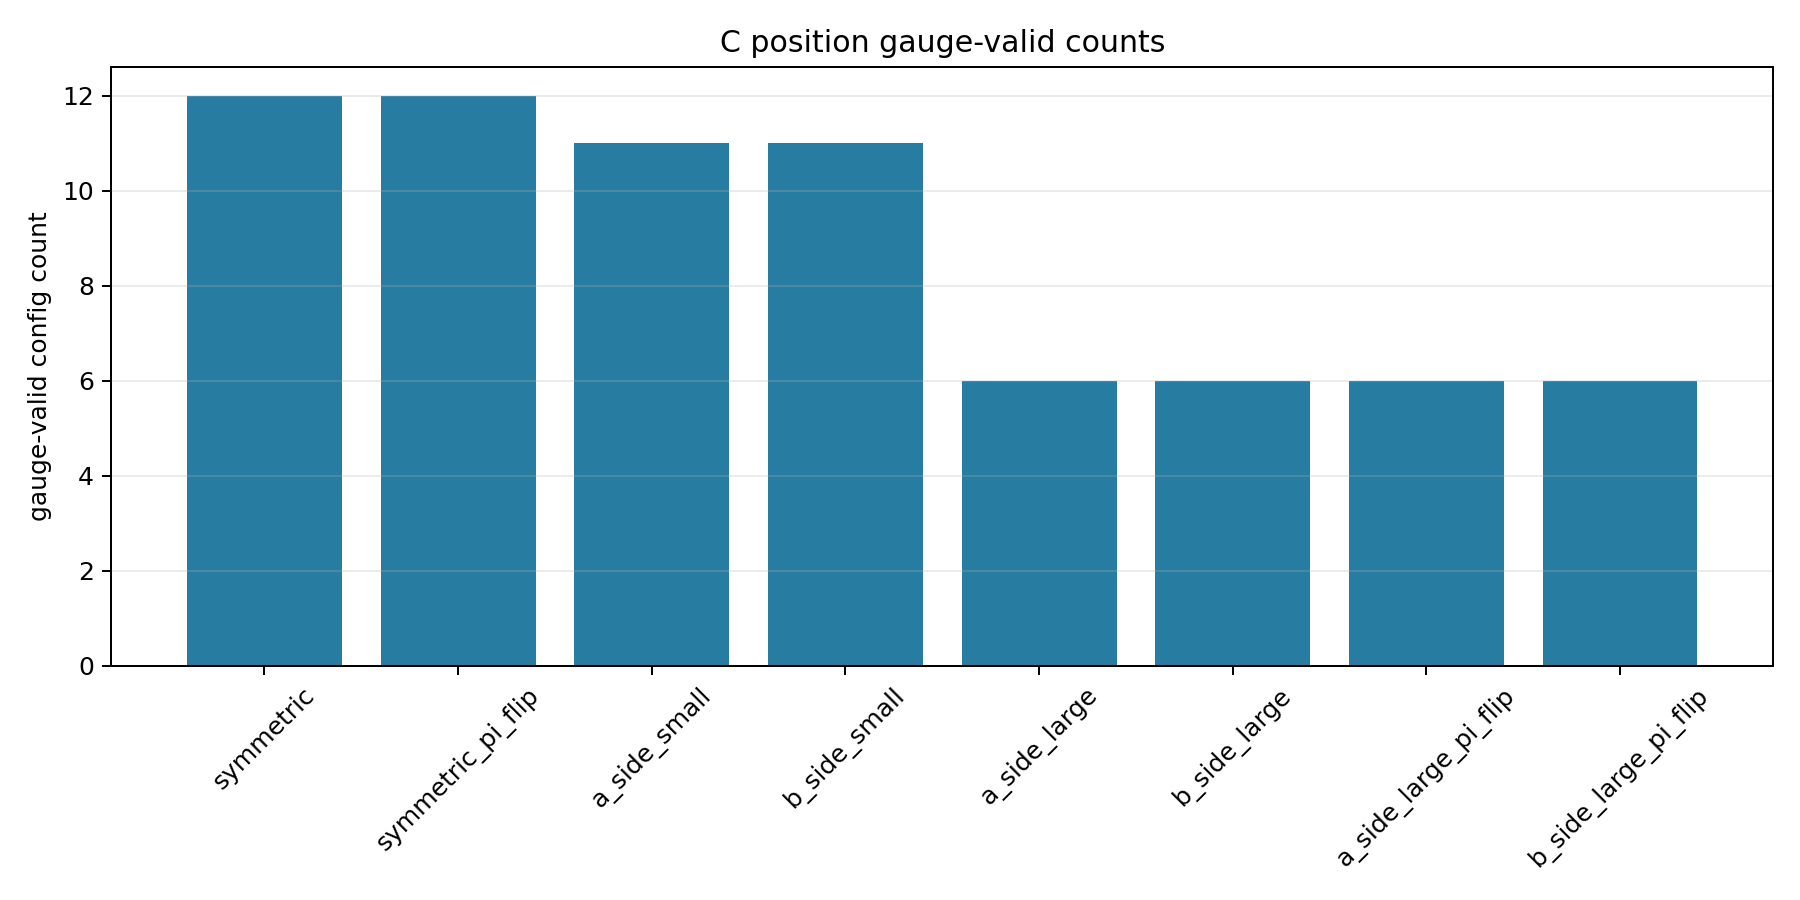
\includegraphics[keepaspectratio]{abc_c_gauge_ab_distance_exponent_c_position_control_preliminary_result_v1/abc_c_gauge_c_position_valid_counts_v1.png}}
&
\pandocbounded{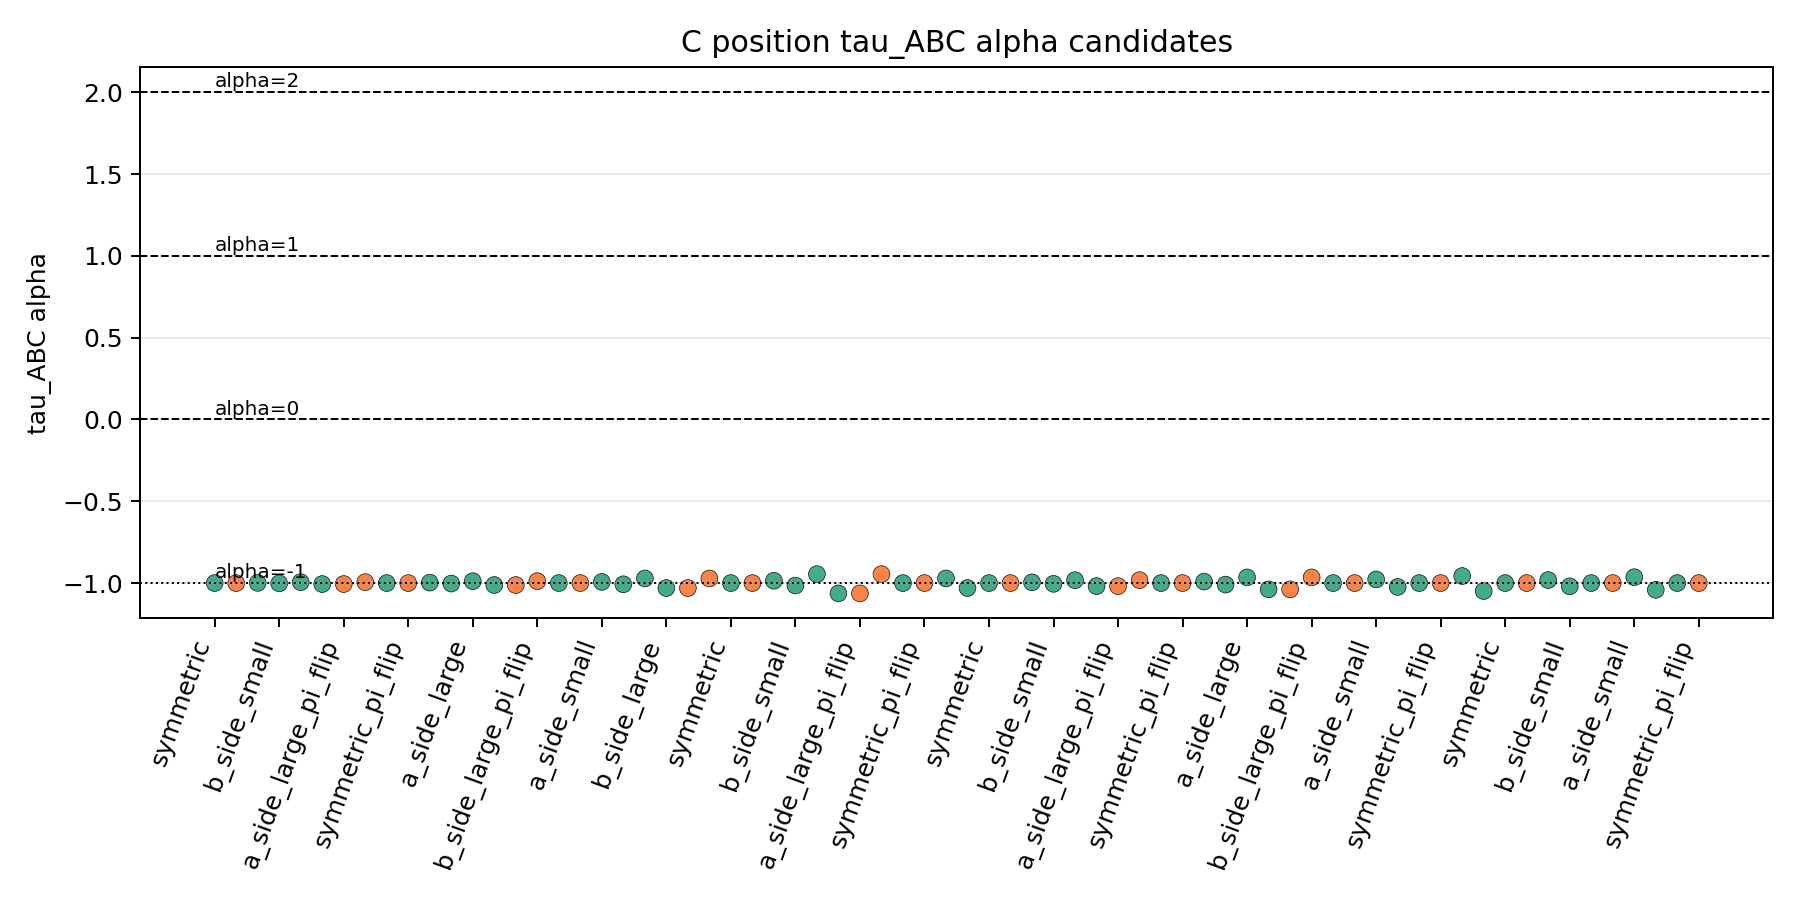
\includegraphics[keepaspectratio]{abc_c_gauge_ab_distance_exponent_c_position_control_preliminary_result_v1/abc_c_gauge_c_position_alpha_candidates_v1.png}} \\
\end{longtable}
}

{\def\LTcaptype{none} % do not increment counter
\begin{longtable}[]{@{}
  >{\raggedright\arraybackslash}p{(\linewidth - 0\tabcolsep) * \real{1.0000}}@{}}
\toprule\noalign{}
\begin{minipage}[b]{\linewidth}\raggedright
A-side/B-side symmetry
\end{minipage} \\
\midrule\noalign{}
\endhead
\bottomrule\noalign{}
\endlastfoot
\pandocbounded{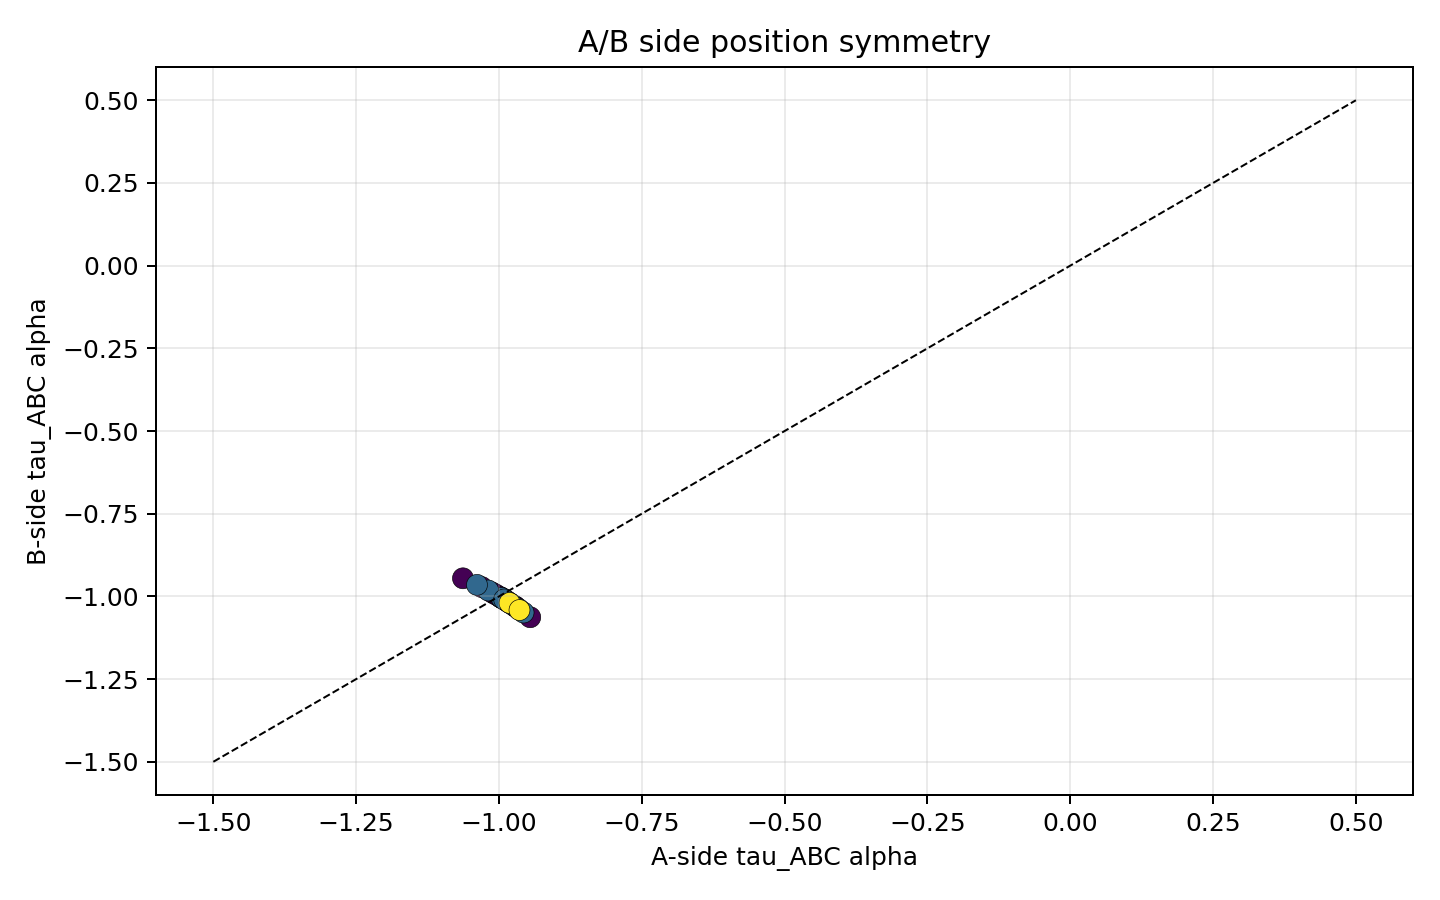
\includegraphics[keepaspectratio]{abc_c_gauge_ab_distance_exponent_c_position_control_preliminary_result_v1/abc_c_gauge_c_position_pair_symmetry_v1.png}} \\
\end{longtable}
}

\begin{center}\rule{0.5\linewidth}{0.5pt}\end{center}

\subsection{4. Relational Compensation
Decomposition}\label{relational-compensation-decomposition}

\subsubsection{4.1 Meaning of the
Experiment}\label{meaning-of-the-experiment-2}

In the ABC three-body system, the relations separate into at least four:

\begin{Shaded}
\begin{Highlighting}[]
\NormalTok{f\_AB}
\NormalTok{f\_AC}
\NormalTok{f\_BC}
\NormalTok{f\_ABC}
\end{Highlighting}
\end{Shaded}

The main target is \texttt{f\_AB}.

\texttt{f\_AC} and \texttt{f\_BC} are the C-derived two-body relations.

\texttt{f\_ABC} is the common relation of the whole ABC system.

The experiment tested the following separation:

\begin{Shaded}
\begin{Highlighting}[]
\NormalTok{representative time: tau\_ABC}
\NormalTok{circumferential{-}direction candidates: f\_AB, f\_AC, f\_BC}
\NormalTok{common{-}mode or central{-}direction candidate: f\_ABC}
\end{Highlighting}
\end{Shaded}

Especially important is the discipline:

\begin{Shaded}
\begin{Highlighting}[]
\NormalTok{Use f\_ABC as representative time.}
\NormalTok{Do not directly add f\_ABC to the AB circumferential direction.}
\end{Highlighting}
\end{Shaded}

\subsubsection{4.2 Main Result}\label{main-result-2}

{\def\LTcaptype{none} % do not increment counter
\begin{longtable}[]{@{}lr@{}}
\toprule\noalign{}
Quantity & Value \\
\midrule\noalign{}
\endhead
\bottomrule\noalign{}
\endlastfoot
\texttt{config\_count} & \texttt{240} \\
\texttt{decomposition\_valid\_count} & \texttt{180} \\
\texttt{AB\_dominant\_valid\_count} & \texttt{48} \\
\texttt{non\_AB\_dominant\_count} & \texttt{132} \\
\texttt{inverse\_or\_inverse\_square\_in\_AB\_dominant\_count} &
\texttt{0} \\
\end{longtable}
}

The \texttt{tau\_ABC} distance-exponent classification in AB-dominant
cases was:

\begin{Shaded}
\begin{Highlighting}[]
\NormalTok{proportional\_like\_alpha\_minus1: 48}
\end{Highlighting}
\end{Shaded}

The native \texttt{f\_AB} classification was:

\begin{Shaded}
\begin{Highlighting}[]
\NormalTok{proportional\_like\_alpha\_minus1: 180}
\end{Highlighting}
\end{Shaded}

The C-bias and C-asymmetry terms were read mainly as

\begin{Shaded}
\begin{Highlighting}[]
\NormalTok{constant\_like\_alpha0.}
\end{Highlighting}
\end{Shaded}

This indicates that the C-derived projection bias did not appear as a
stable inverse-law or inverse-square term with respect to AB distance
\texttt{L\_AB}.

\subsubsection{4.3 Direct-Addition Control for
f\_ABC}\label{direct-addition-control-for-f_abc}

In the erroneous direct-injection control where \texttt{f\_ABC} was
directly added to the AB circumferential direction, the result was:

\begin{Shaded}
\begin{Highlighting}[]
\NormalTok{other: 63}
\NormalTok{proportional\_like\_alpha\_minus1: 117}
\end{Highlighting}
\end{Shaded}

This shows that treating \texttt{f\_ABC} as a causal term in the AB
circumferential direction muddies the classification.

At this stage, therefore, the following separation is appropriate:

\begin{Shaded}
\begin{Highlighting}[]
\NormalTok{Use f\_ABC as representative time tau\_ABC.}
\NormalTok{Do not directly add f\_ABC to the AB circumferential direction.}
\end{Highlighting}
\end{Shaded}

This does not mean that \texttt{f\_ABC} is ignored.

\texttt{f\_ABC} is recorded as the common mode or central-direction
compensation of the whole system.

\subsubsection{4.4 Figures}\label{figures-2}

{\def\LTcaptype{none} % do not increment counter
\begin{longtable}[]{@{}
  >{\raggedright\arraybackslash}p{(\linewidth - 2\tabcolsep) * \real{0.5000}}
  >{\raggedright\arraybackslash}p{(\linewidth - 2\tabcolsep) * \real{0.5000}}@{}}
\toprule\noalign{}
\begin{minipage}[b]{\linewidth}\raggedright
Decomposition valid count
\end{minipage} & \begin{minipage}[b]{\linewidth}\raggedright
Pair alpha
\end{minipage} \\
\midrule\noalign{}
\endhead
\bottomrule\noalign{}
\endlastfoot
\pandocbounded{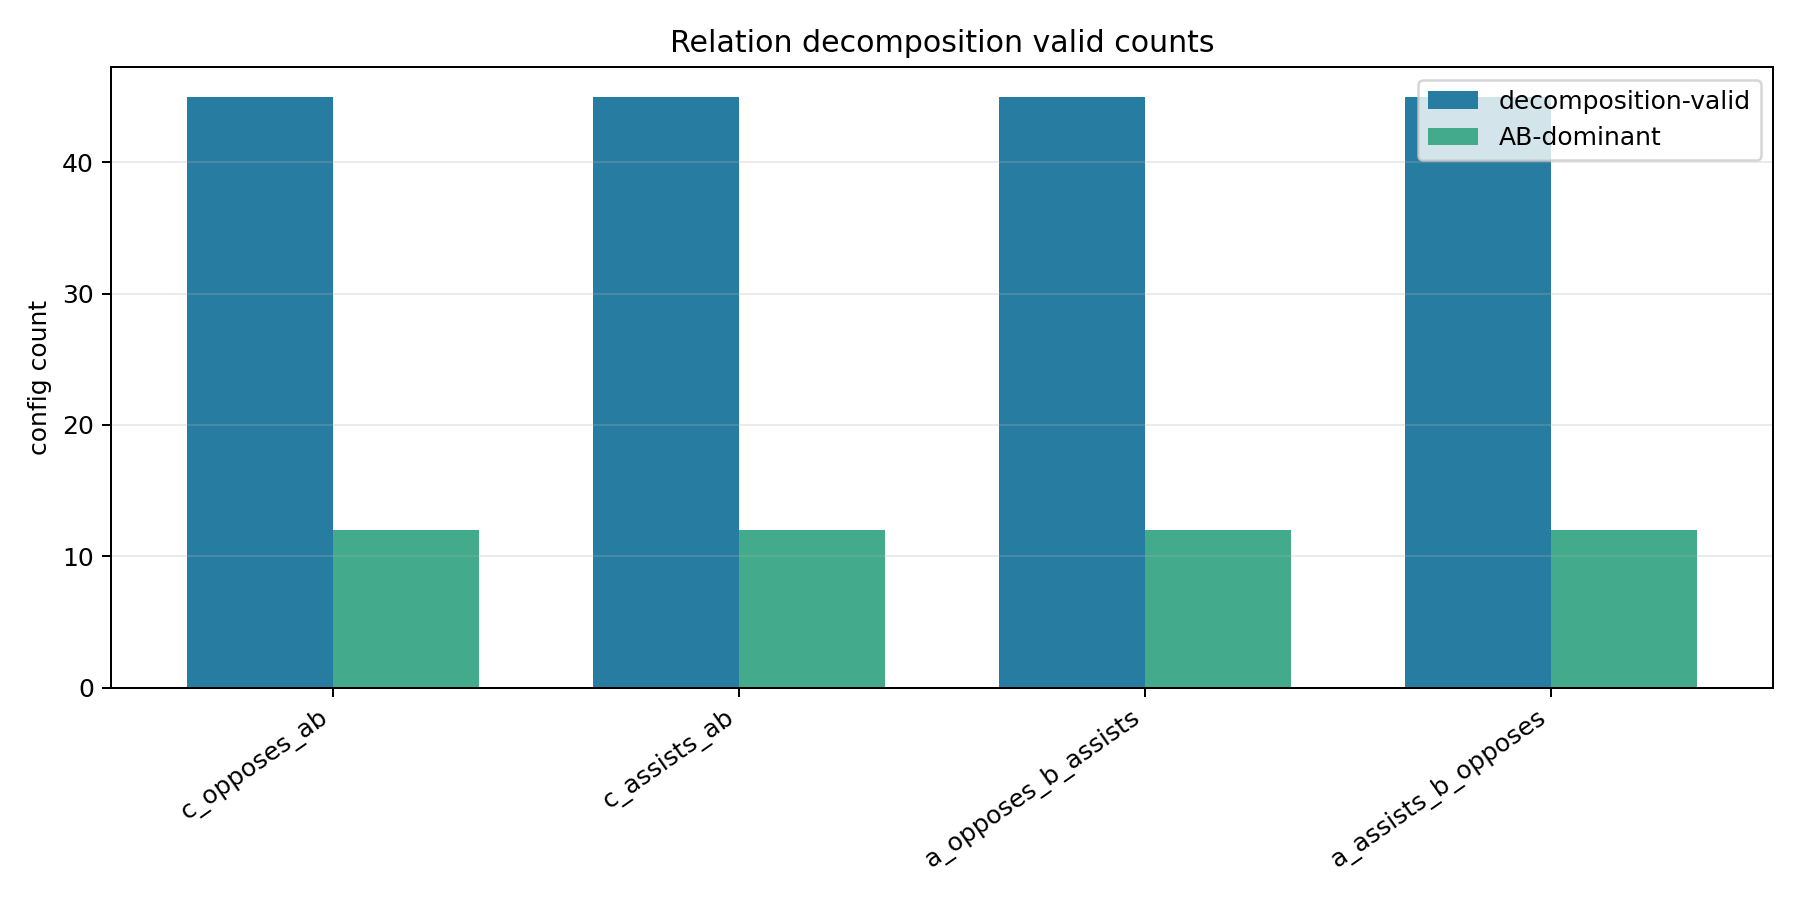
\includegraphics[keepaspectratio]{abc_c_gauge_relation_decomposition_preliminary_result_v1/abc_c_gauge_relation_decomposition_valid_counts_v1.png}}
&
\pandocbounded{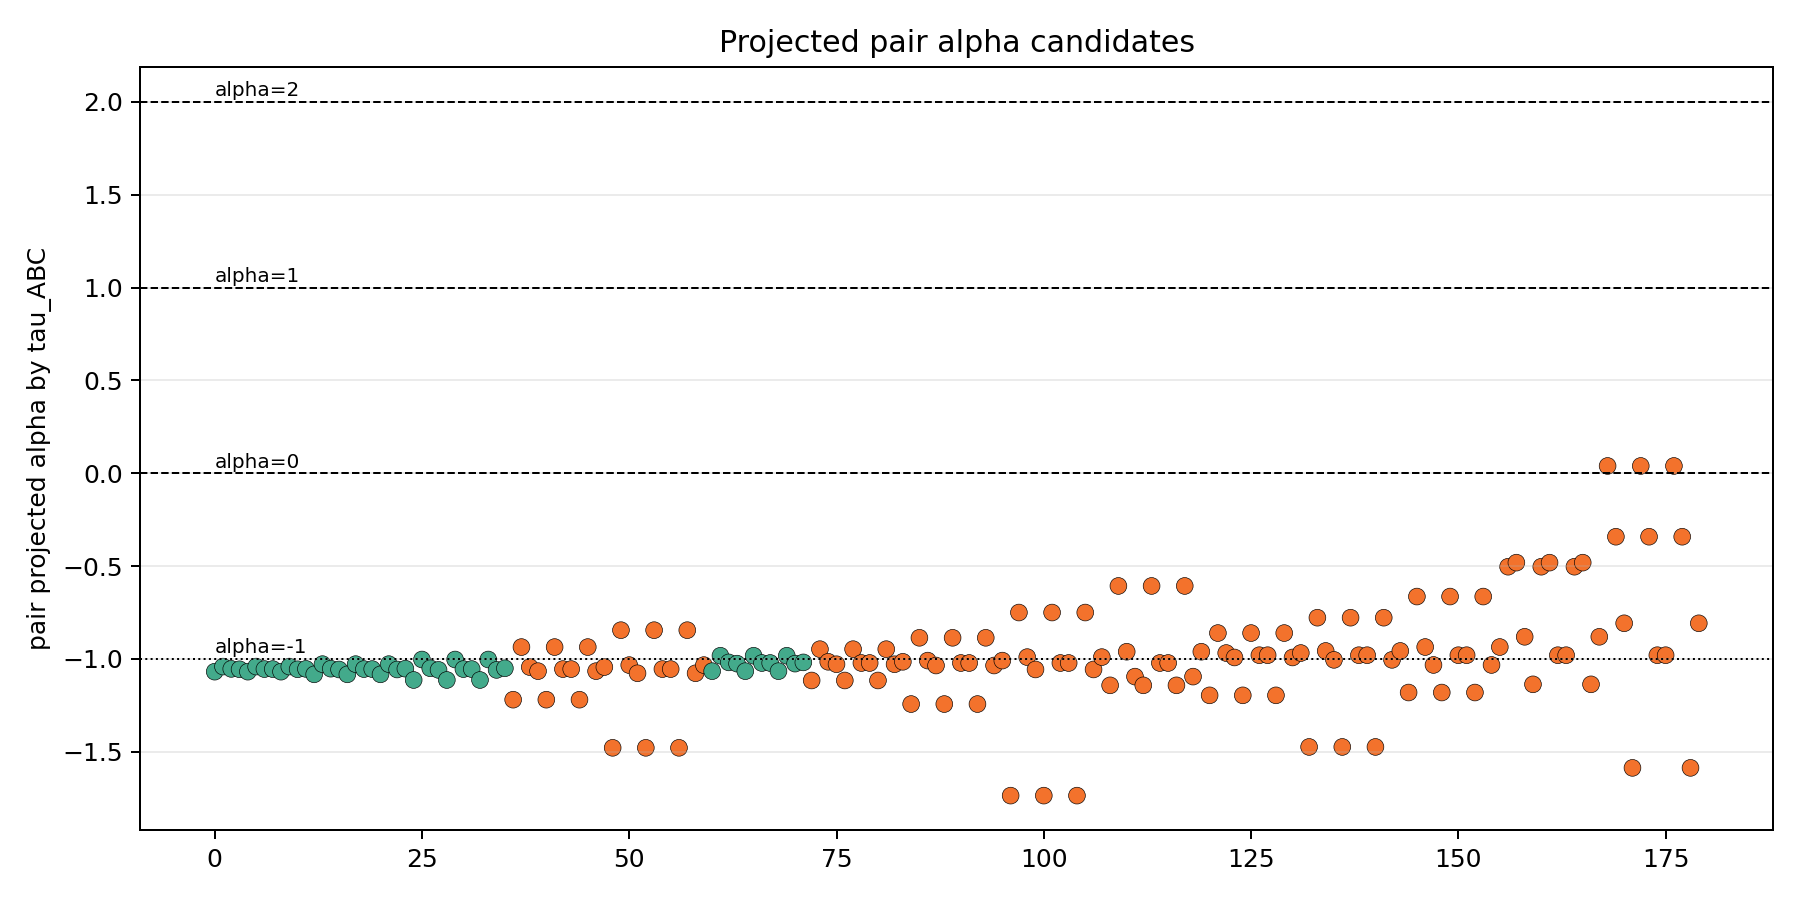
\includegraphics[keepaspectratio]{abc_c_gauge_relation_decomposition_preliminary_result_v1/abc_c_gauge_relation_decomposition_pair_alpha_v1.png}} \\
\end{longtable}
}

{\def\LTcaptype{none} % do not increment counter
\begin{longtable}[]{@{}
  >{\raggedright\arraybackslash}p{(\linewidth - 2\tabcolsep) * \real{0.5000}}
  >{\raggedright\arraybackslash}p{(\linewidth - 2\tabcolsep) * \real{0.5000}}@{}}
\toprule\noalign{}
\begin{minipage}[b]{\linewidth}\raggedright
Native / pair comparison
\end{minipage} & \begin{minipage}[b]{\linewidth}\raggedright
C-contamination diagnosis
\end{minipage} \\
\midrule\noalign{}
\endhead
\bottomrule\noalign{}
\endlastfoot
\pandocbounded{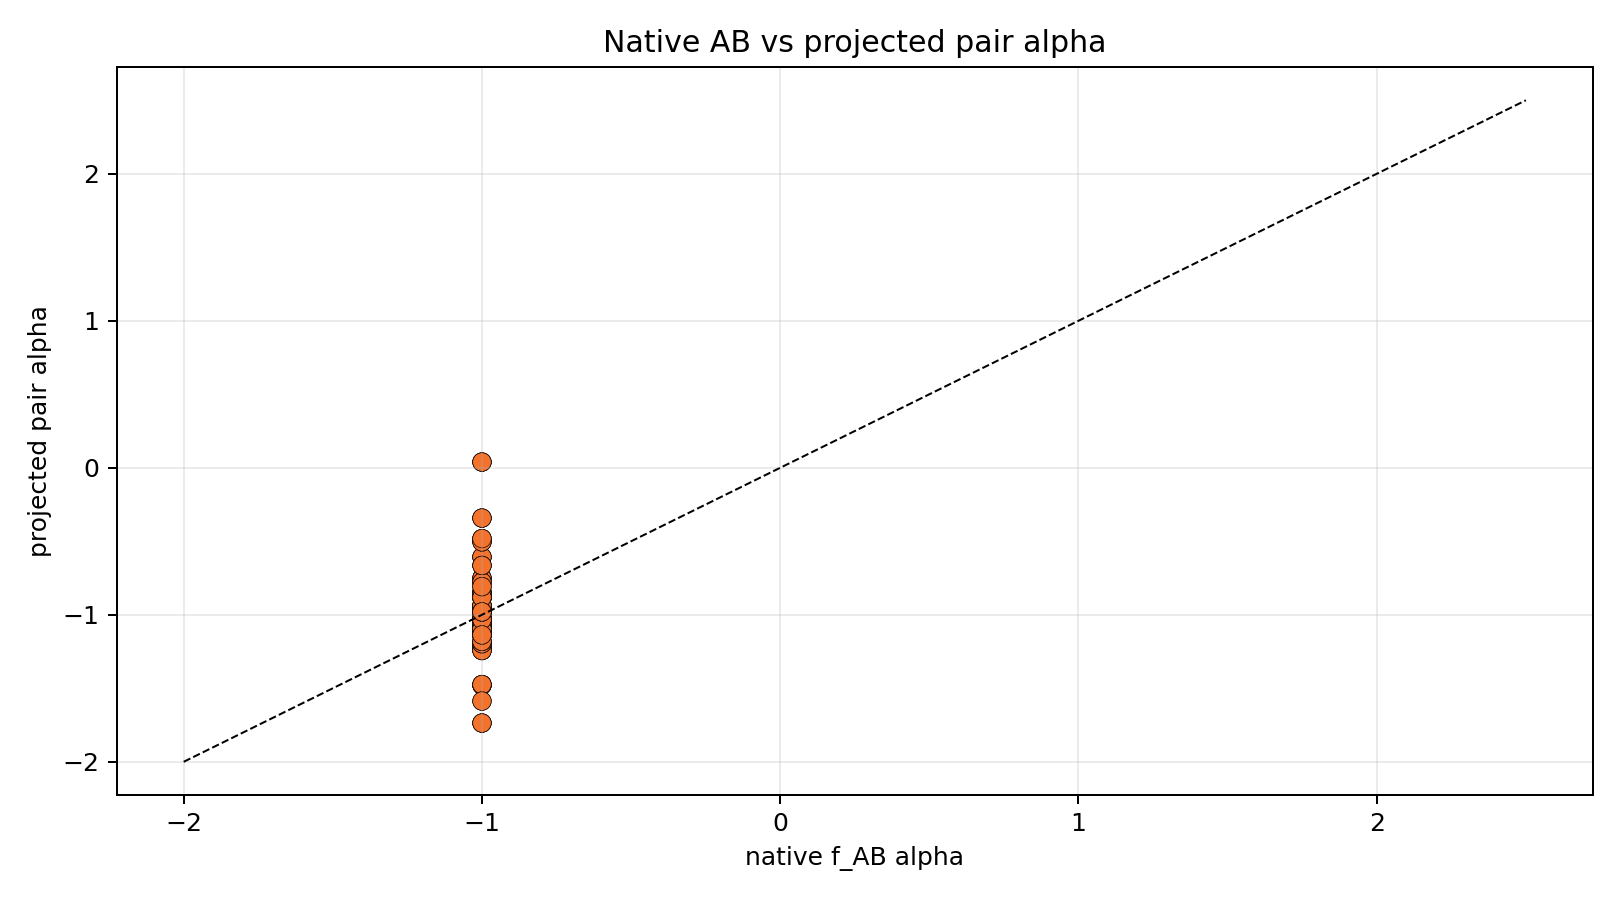
\includegraphics[keepaspectratio]{abc_c_gauge_relation_decomposition_preliminary_result_v1/abc_c_gauge_relation_decomposition_native_vs_pair_alpha_v1.png}}
&
\pandocbounded{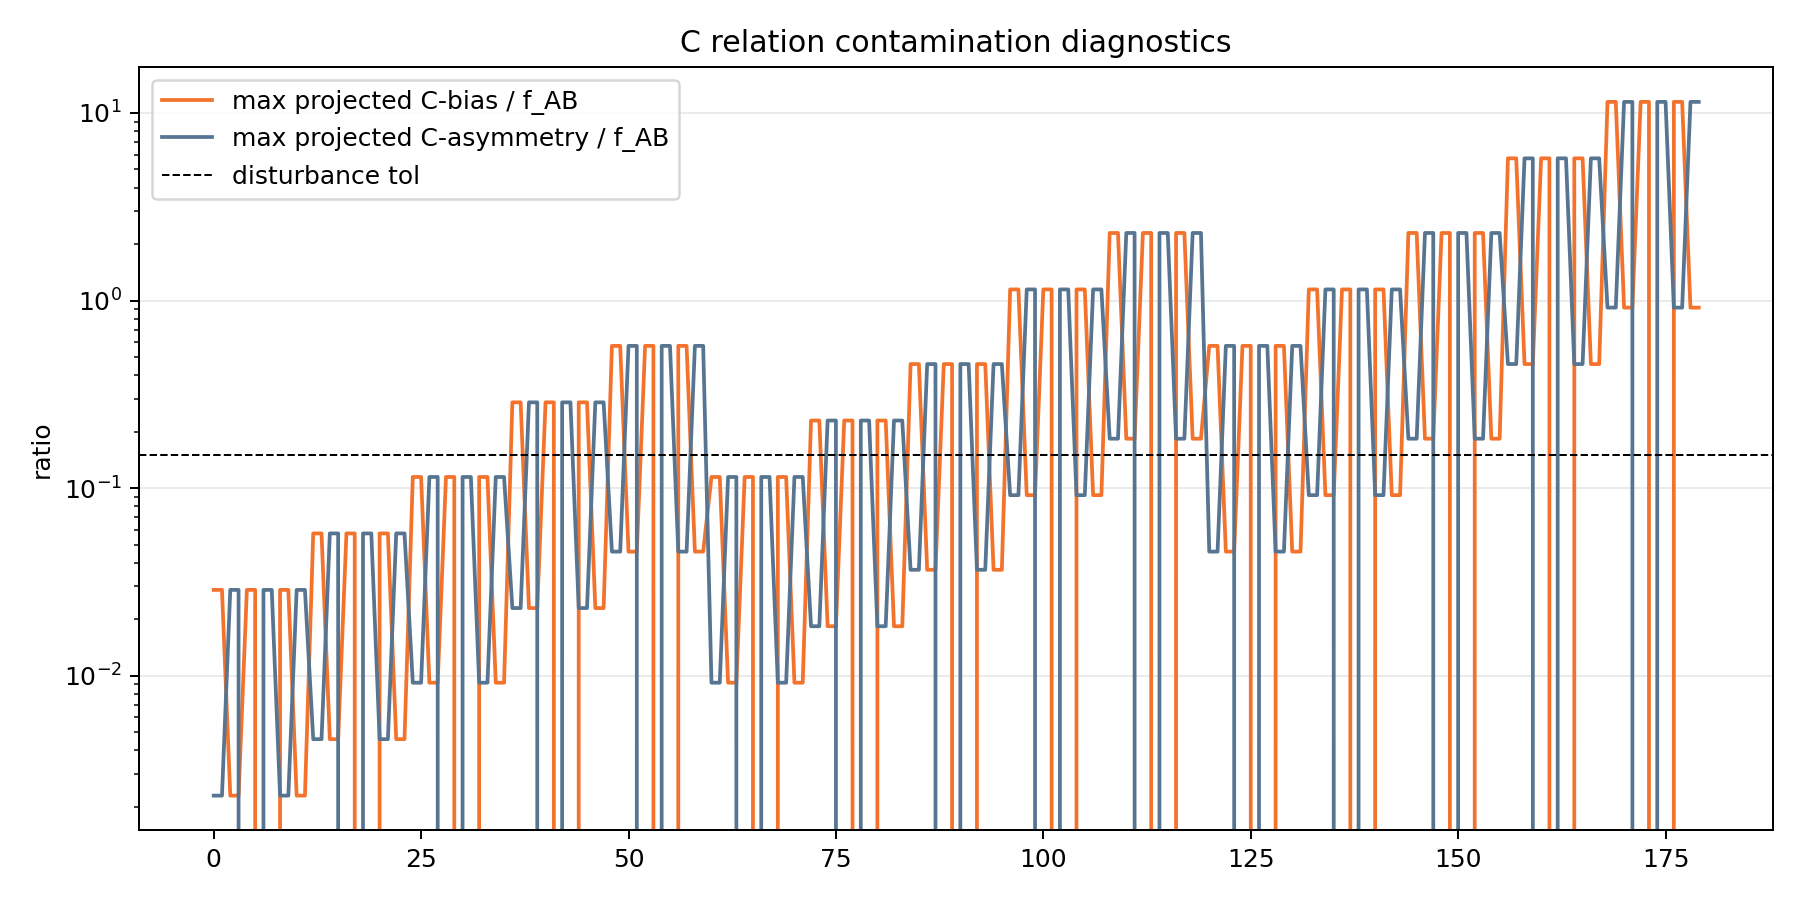
\includegraphics[keepaspectratio]{abc_c_gauge_relation_decomposition_preliminary_result_v1/abc_c_gauge_relation_decomposition_contamination_v1.png}} \\
\end{longtable}
}

\begin{center}\rule{0.5\linewidth}{0.5pt}\end{center}

\subsection{5. Overall Judgment}\label{overall-judgment}

\subsubsection{5.1 Established}\label{established}

{\def\LTcaptype{none} % do not increment counter
\begin{longtable}[]{@{}
  >{\raggedright\arraybackslash}p{(\linewidth - 2\tabcolsep) * \real{0.5000}}
  >{\raggedright\arraybackslash}p{(\linewidth - 2\tabcolsep) * \real{0.5000}}@{}}
\toprule\noalign{}
\begin{minipage}[b]{\linewidth}\raggedright
Item
\end{minipage} & \begin{minipage}[b]{\linewidth}\raggedright
Judgment
\end{minipage} \\
\midrule\noalign{}
\endhead
\bottomrule\noalign{}
\endlastfoot
C gauge has a valid window & Established \\
Too small \texttt{R\_C} makes cells too coarse & Confirmed \\
Too strong or biased C causes gauge contamination & Confirmed \\
Discipline of reading \texttt{tau\_ABC} as representative time &
Supported \\
Need to record \texttt{tau\_AB}, \texttt{tau\_AC}, and \texttt{tau\_BC}
as auxiliary diagnostics & Confirmed \\
Separation of \texttt{f\_AB}, \texttt{f\_AC}, \texttt{f\_BC}, and
\texttt{f\_ABC} & Supported \\
Discipline of not directly adding \texttt{f\_ABC} in the circumferential
direction & Supported \\
\end{longtable}
}

\subsubsection{5.2 Not Established}\label{not-established}

{\def\LTcaptype{none} % do not increment counter
\begin{longtable}[]{@{}
  >{\raggedright\arraybackslash}p{(\linewidth - 2\tabcolsep) * \real{0.5000}}
  >{\raggedright\arraybackslash}p{(\linewidth - 2\tabcolsep) * \real{0.5000}}@{}}
\toprule\noalign{}
\begin{minipage}[b]{\linewidth}\raggedright
Item
\end{minipage} & \begin{minipage}[b]{\linewidth}\raggedright
Judgment
\end{minipage} \\
\midrule\noalign{}
\endhead
\bottomrule\noalign{}
\endlastfoot
Inverse-law form appears from C gauge alone & Not detected \\
Inverse-square form appears from C gauge alone & Not detected \\
Changing C position alone changes the exponent law & Not detected \\
C-derived terms become inverse-law or inverse-square terms of AB
distance & Not detected \\
Present minimal AB harmonic model becomes standard-gravity type & Not
established \\
\end{longtable}
}

\begin{center}\rule{0.5\linewidth}{0.5pt}\end{center}

\subsection{6. Interpretation}\label{interpretation}

The most important consequence of this experiment group is:

\begin{Shaded}
\begin{Highlighting}[]
\NormalTok{Even after returning to an ABC three{-}body system, the current minimal model is read as proportional{-}type.}
\end{Highlighting}
\end{Shaded}

This is not a negative failure.

It is a boundary condition: the acceleration-like readout obtained in
the AB two-body system was re-read using the independent metric C, but
it was not transformed into an inverse-law or inverse-square-law form.

The AB two-body system lacked an independent gauge.

The ABC three-body system introduced the independent metric C, but since
C itself is part of the closed phase system,

\begin{Shaded}
\begin{Highlighting}[]
\NormalTok{f\_AC}
\NormalTok{f\_BC}
\NormalTok{f\_ABC}
\end{Highlighting}
\end{Shaded}

arise.

Even after separating these terms, AB-dominant cases preserved the
proportional type.

Therefore, the current model essentially behaves as

\begin{Shaded}
\begin{Highlighting}[]
\NormalTok{a one{-}dimensional relative{-}phase displacement model.}
\end{Highlighting}
\end{Shaded}

Within that scope, inverse-law and inverse-square-law forms do not arise
naturally.

The result shows that the distance-exponent problem cannot be solved
merely by adding C.

Increasing the strength of C improves metric resolution, but increases
contamination by \texttt{f\_AC}, \texttt{f\_BC}, and \texttt{f\_ABC}.

Weakening C reduces contamination, but the cell resolution becomes
insufficient for reading changes in the position phase difference.

Thus, C gauge has a valid window, but that window was not a mechanism
for converting the present one-dimensional harmonic model into an
inverse-square form.

\begin{center}\rule{0.5\linewidth}{0.5pt}\end{center}

\subsection{7. Deferred Problems}\label{deferred-problems}

\subsubsection{7.1 The Inverse Square Is Not Generally
Denied}\label{the-inverse-square-is-not-generally-denied}

The present experiment denies only the narrow claim:

\begin{Shaded}
\begin{Highlighting}[]
\NormalTok{If C gauge and relational decomposition are added to the present minimal AB harmonic model,}
\NormalTok{an inverse{-}law or inverse{-}square form appears natively.}
\end{Highlighting}
\end{Shaded}

This claim was not supported.

However, this does not show that inverse-square forms are absent from
closed phase systems in general.

\subsubsection{7.2 Reason for Not Performing Three- or Four-Dimensional
Extensions}\label{reason-for-not-performing-three--or-four-dimensional-extensions}

To explain the inverse-square form in a standard way, a structure such
as area sweep or spherical-shell sweep seems necessary.

Therefore, experiments increasing position-phase degrees of freedom to
three or four dimensions were considered.

However, the present experiment system is a model in which two localized
waves harmonically oscillate in the relative phase direction.

Even if this structure is made higher-dimensional, projection onto a
geodesic or two-dimensional section returns to the same two-body
harmonic readout as in this experiment.

Therefore, within this model, three- or four-dimensional extension is
unlikely to newly produce inverse-law or inverse-square behavior.

For this reason, the higher-dimensional extension experiment was not
performed in this series.

\subsubsection{7.3 Circular Waves, Spherical Waves, and Limited
Connection to the Double-Slit
Papers}\label{circular-waves-spherical-waves-and-limited-connection-to-the-double-slit-papers}

In the observational principle of this series, however, what can be
observed is a localized wave. A merely conceptual extended circular wave
cannot simply be placed as a real entity.

If one assumes a circular or spherical-shell wave, it appears easy to
construct an area sweep or inverse-square form.

However, such a wave is broadly extended in both spatial and temporal
phase directions, and it becomes unclear by which local readout its
position phase and temporal phase are measured.

Therefore, at present, the circular-wave or spherical-shell-wave model
is suspended not because it is impossible to experiment with, but
because it may contain an excessive reality assumption relative to the
observational principle.

When referring here to the double-slit thought-experiment series, the
scope of citation must be limited.

The first paper in that series showed that, when a position fluctuation
\texttt{P(y)} is given to a stationary single-wavelength point light
source, each far-field interference fringe retains its shape and shifts
only by the geometric path difference; repeated trials push the
distribution of fringe shifts forward from \texttt{P(y)}.

As a concrete example, when \texttt{P(y)=cos\^{}2} is placed, the
\texttt{cos\^{}2} form is preserved under a near-axis linear map, and
non-near-axis deviation appears as several-percent geometric
nonlinearity.

However, that paper treats an observation mode in which the fringe shift
is read in each trial. It is separate from the visibility-reduction mode
that integrates many-trial intensities into one image.

The second paper in that series extended this pushed-forward readout to
a localized odd-harmonic source.

There, a localized odd-harmonic source can preserve its shape and appear
in the double-slit far field only under alignment conditions, and under
position fluctuation the shape preservation becomes fragile due to
off-axis scattering.

The single-wavelength case \texttt{N=1} has no such fragility and was
confirmed as a special case that agrees with the first paper to machine
precision.

Thus, the implication that can be correctly carried from the double-slit
papers to the present paper is limited to the following research
direction.

From this viewpoint, rather than placing an extended probability wave or
spherical wave directly as real, it is closer to the observational
principle of this series to examine whether

\begin{Shaded}
\begin{Highlighting}[]
\NormalTok{many observations of localized waves,}
\NormalTok{initial{-}position or phase fluctuation,}
\NormalTok{and the push{-}forward of that fluctuation to the observation side}
\end{Highlighting}
\end{Shaded}

can appear as a broadened statistical image or area distribution.

This is not a proposition directly proven by the double-slit papers.

What those papers showed is only that a position-fluctuation
distribution is pushed forward into a distribution of fringe shifts, and
that extension to localized sources adds alignment conditions and
fragility of shape preservation.

Therefore, instead of

\begin{Shaded}
\begin{Highlighting}[]
\NormalTok{assuming an extended wave,}
\end{Highlighting}
\end{Shaded}

the next question should be:

\begin{Shaded}
\begin{Highlighting}[]
\NormalTok{Can many{-}trial, many{-}initial{-}condition readout of localized waves appear statistically as area broadening?}
\end{Highlighting}
\end{Shaded}

That question exceeds the scope of this experiment series and is
deferred here.

\begin{center}\rule{0.5\linewidth}{0.5pt}\end{center}

\subsection{8. How This Series Should Be
Closed}\label{how-this-series-should-be-closed}

It is reasonable to close this series with the following results.

\begin{Shaded}
\begin{Highlighting}[]
\NormalTok{In the AB two{-}body system, harmonic readout and chi{-}tau area can be read.}
\NormalTok{However, there is not enough independent gauge structure to determine the distance exponent.}

\NormalTok{In the ABC three{-}body system, C gauge and relational decomposition can be introduced.}
\NormalTok{However, in the present minimal model the proportional type is preserved,}
\NormalTok{and inverse{-}law or inverse{-}square forms do not appear natively.}

\NormalTok{Therefore, the inverse{-}square problem must be redesigned not as a simple extension}
\NormalTok{of this one{-}dimensional closed phase model, but as a problem of observational statistics,}
\NormalTok{area readout, localized{-}wave ensembles, and push{-}forward maps of initial fluctuations.}
\end{Highlighting}
\end{Shaded}

\begin{center}\rule{0.5\linewidth}{0.5pt}\end{center}

\section{References}\label{references}

\subsection{Self-References}\label{self-references}

\begin{enumerate}
\def\labelenumi{\arabic{enumi}.}
\tightlist
\item
  Noriaki Kihara, ``Basic Axiom System of the Nameless Equal-Amplitude
  Composite Wave Model v4'', Version DOI:
  \texttt{10.5281/zenodo.21316620}, Concept DOI:
  \texttt{10.5281/zenodo.21315735}, 2026.
\item
  Noriaki Kihara, ``Construction Experiment of Multigauge Interference
  Readout Conserved Quantities in an ABC Closed Phase System'', Version
  DOI: \texttt{10.5281/zenodo.21308050}, Concept DOI:
  \texttt{10.5281/zenodo.21308049}, 2026.
\item
  Noriaki Kihara, ``Preliminary Summary of Harmonic Readout and c=1 Area
  Sweep in an AB Two-Body Closed Phase System'', Version DOI:
  \texttt{10.5281/zenodo.21318697}, Concept DOI:
  \texttt{10.5281/zenodo.21318696}, 2026.
\item
  Noriaki Kihara,
  \href{ABC閉鎖位相系における独立計量CによるAB関係補償の距離指数読出し実験仕様書\%20v1.md}{Experiment
  Specification for Distance-Exponent Readout of AB Relational
  Compensation Using Independent Metric C in an ABC Closed Phase System
  v1}, 2026.
\item
  Noriaki Kihara,
  \href{閉鎖複素位相波における自己項の内部閉鎖とN体外部読出し分離に関する定義補足.md}{Definitional
  Supplement on Internal Closure of Self-Terms and Separation of N-Body
  External Readout in Closed Complex Phase Waves}, 2026.
\item
  Noriaki Kihara, ``Double-Slit Interference Thought Experiment with a
  Source Having Position Fluctuation: Push-Forward of Source Position
  Distribution to Fringe-Shift Distribution (Shape Preservation)'',
  Version DOI: \texttt{10.5281/zenodo.21035809}, Concept DOI:
  \texttt{10.5281/zenodo.21035808}, 2026.
\item
  Noriaki Kihara, ``Double-Slit Interference Thought Experiment with a
  Localized Odd-Harmonic Source: Shape Preservation Is Conditional and
  Fragile, and the Single-Wavelength Case N=1 Is a Robust Special
  Case'', Version DOI: \texttt{10.5281/zenodo.21035831}, Concept DOI:
  \texttt{10.5281/zenodo.21035830}, 2026.
\end{enumerate}

\subsection{External References}\label{external-references}

The external references are used only as minimal standard background on
distance laws, relativistic time, and phase readout, not as derivational
premises of this paper.

\begin{enumerate}
\def\labelenumi{\arabic{enumi}.}
\setcounter{enumi}{7}
\tightlist
\item
  Isaac Newton, \emph{Philosophiae Naturalis Principia Mathematica},
  1687.
\item
  Albert Einstein, ``Die Grundlage der allgemeinen
  Relativitaetstheorie'', \emph{Annalen der Physik} 49, 769-822, 1916.
  DOI: \texttt{10.1002/andp.19163540702}.
\item
  Y. Aharonov and D. Bohm, ``Significance of electromagnetic potentials
  in the quantum theory'', \emph{Physical Review} 115, 485-491, 1959.
  DOI: \texttt{10.1103/PhysRev.115.485}.
\end{enumerate}

\end{document}
